%\documentclass[tikz, border=5pt]{standalone}
\begin{document}
	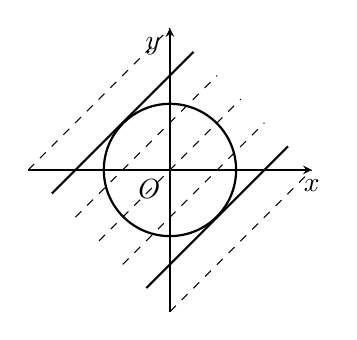
\begin{tikzpicture}[>=stealth, scale=0.6] % 缩放使图形更清晰
		% 1. 绘制坐标轴
		\draw[->] (-3,0) -- (3,0) node[below] {$x$};
		\draw[->] (0,-3) -- (0,3) node[below left] {$y$};
		\node at (0,0) [below left] {$O$};  % 原点标记
		
		% 绘制圆
		\draw[thick] (0,0) circle (1.4);
		
		% 绘制线
		\draw[thick] (-0.5, -2.5) -- (2.5, 0.5) ; 
		\draw[thick] (-2.5, -0.5) -- (0.5, 2.5) ; 
		
		% 绘制虚线
		\draw[dashed] (-2, -1) -- (1, 2) ; 
		\draw[dashed] (-1.5, -1.5) -- (1.5, 1.5) ; 
		\draw[dashed] (-1, -2) -- (2, 1) ; 
		\draw[dashed] (-3,0) -- (0,3); 
		\draw[dashed] (0,-3) -- (3,0); 
		
	\end{tikzpicture}
\end{document}
